% !TeX program = lualatex
\documentclass[fleqn]{NotesClass}

\strictpagecheck

\usepackage{csquotes}

\usepackage{tikz}
\usetikzlibrary{external}
\tikzexternalize[prefix=tikz-external/]

\usepackage{tikz-cd}
\AtBeginEnvironment{tikzcd}{\tikzexternaldisable}
\AtEndEnvironment{tikzcd}{\tikzexternalenable}

\usepackage[pdfauthor={Willoughby Seago},pdftitle={Notes from Solitons Course},pdfkeywords={soliton, kdv equation},pdfsubject={solitons}]{hyperref}  % Should be loaded second last (cleveref last)
\colorlet{hyperrefcolor}{blue!60!black}
\hypersetup{colorlinks=true, linkcolor=hyperrefcolor, urlcolor=hyperrefcolor}
\usepackage[
capitalize,
nameinlink,
noabbrev
]{cleveref} % Should be loaded last

% My packages
\usepackage{NotesBoxes}
\usepackage{NotesMaths2}

\setmathfont[range={\int, \oint, \otimes, \oplus, \bigotimes, \bigoplus}]{Latin Modern Math}


% Highlight colour
\definecolor{highlight}{HTML}{D61C27}
\definecolor{my blue}{HTML}{BBDBDA}
%\definecolor{my red}{HTML}{770D38}
%\definecolor{my green}{HTML}{14770D}
%\definecolor{my yellow}{HTML}{E7BB41}

% Title page info
\title{Solitons}
\author{Willoughby Seago}
\date{January 13th, 2024}
\subtitle{Notes from}
\subsubtitle{University of Glasgow}
\renewcommand{\abstracttext}{These are my notes from the master's course \emph{Solitons} taught at the University of Glasgow by Prof Ian Strachan. These notes were last updated at \printtime{} on \today{}.}

% Commands
% Maths
\renewcommand{\dl}{\symrm{d}}
\renewcommand{\dd}{\,\symrm{d}}
\newcommand{\groupVelocity}{c_{\symrm{g}}}
\DeclareMathOperator{\sech}{sech}
\newcommand{\const}{\symrm{const}}


\begin{document}
    \frontmatter
    \titlepage
    \innertitlepage{images/breaking-wave}
    \tableofcontents
    % \listoffigures
    \mainmatter
    \chapter{Introduction}
    This course will study solitons.
    These are certain solutions to nonlinear partial differential equations posessing certain properties.
    The key one being that they are localised and at large separations different solitons behave independently of each other.
    
    We will focus on one spatial dimension for most of our equations, although many have generalisations to more spatial dimensions.
    
    We are focused on when solutions exist, so we'll ignore edge cases and make necessary assumptions.
    In particular any \enquote{arbitrary} function will be assumed to be sufficiently differentiable and integrable for any required derivatives or integrals to exist.
    
    This is a maths course, not a physics course, so we will include a minimal number of constants.
    Equations with more constants can be brought into the standard form of the equation with a minimal number of constants by redefining parameters.
    
    \section{Notation}
    If \(u\) is a function of some variable, say \(\xi\), then we write
    \begin{equation}
        u_\xi = \diffp{u}{\xi} = \partial_\xi u
    \end{equation}
    for the partial derivative of \(u\) with respect to \(\xi\).
    We extend this notation to multiple derivatives, such as
    \begin{equation}
        u_{\xi\xi} = \diffp[2]{u}{\xi} = \partial_\xi^2 u, \qqand u_{\xi\xi\xi} = \diffp[3]{u}{\xi} = \partial_\xi^3 u.
    \end{equation}
    We also extend this notation to multiple variables, say \(\zeta\), writing, for example,
    \begin{equation}
        u_{\xi\zeta} = \diffp{u}{\zeta,\xi} = \partial_\zeta \partial_\xi u.
    \end{equation}
    
    \chapter{Linear Waves}
    We'll start with a recap of solving linear equations, in particular the wave equation.
    We'll also look at some important properties of solutions.
    
    \section{Linearity}
    Recall that a partial differential equation in \(u\) is \defineindex{linear} if the PDE is linear in \(u\) and its derivatives.
    That means that there are no terms of the form \(u^2\), \(uu_x\), \(u_xu_t\), and so on.
    This is a particularly nice property for many reasons.
    One reason is that linear PDEs are more likely to have solutions that we can find exactly than nonlinear PDEs.
    However, since we're interested in solitons, which are certain solutions to PDEs, this doesn't make much difference as we aren't interested in PDEs without solutions.
    Another reason that linearity is nice is that it gives us the (linear) superposition principle, namely that if \(u_1\) and \(u_2\) are solutions to the PDE then so is \(u_1 + u_2\) and \(A u_1\) for some constant \(A\).
    That is, the solutions form a vector space.
    This lets us write solutions in terms of simpler solutions, and makes the solutions easier to find.
    
    A \defineindex{nonlinear} PDE is one which is not linear.
    Terms like \(uu_x\) break the linear superposition principle, for example, if we have the PDE \(uu_x = 0\) with solutions \(u_1\) and \(u_2\) then substituting \(u_1 + u_2\) into this we get
    \begin{equation}
        (u_1 + u_2) (u_{1x} + u_{2x}) = \underbrace{u_1u_{1x}}_{=0} + u_1u_{2x} + u_2u_{1x} + \underbrace{u_2u_{2x}}_{=0} = u_1u_{2x} + u_2u_{1x},
    \end{equation}
    and this does not vanish in general, so \(u_1 + u_2\) is not a solution.
    
    We emphasise that here we are talking about the \emph{linear} superposition principle, since we shall see in this course that there are sometimes nonlinear ways to combine solutions to a nonlinear PDE and obtain another solution.
    
    \section{Wave Equation}
    One of the first PDEs that we may consider is the \defineindex{wave equation}, which in one spatial dimension takes the form
    \begin{equation}
        u_{tt} - c^2 u_{xx} = 0.
    \end{equation}
    This can be solved by introducing new variables
    \begin{equation}
        X = x - ct, \qand T = x + ct.
    \end{equation}
    The chain rule then tells us that
    \begin{alignat}{3}
        \diffp{}{x} &= \diffp{X}{x} \diffp{}{X} + \diffp{T}{x} \diffp{}{T} &&= \diffp{}{X} + \diffp{}{T},\\
        \diffp{}{t} &= \diffp{X}{t} \diffp{}{X} + \diffp{T}{t} \diffp{}{T} &&= -c\diffp{}{X} + c\diffp{}{T}.
    \end{alignat}
    We then have
    \begin{align}
        u_{xx} &= (\partial_X + \partial_T)^2u\\
        &= (\partial_X + \partial_T)(\partial_X + \partial_T u)\\
        &= \partial_X^2 u + 2\partial_T\partial_X u + \partial_T^2 u
    \end{align}
    and
    \begin{align}
        u_{tt} &= (-c\partial_X + c\partial_T)^2u\\
        &= (-c\partial_X + c\partial_T)(-c\partial_X u + c\partial_T u)\\
        &= c^2 \partial_X^2 u - 2 c^2 \partial_T \partial_X u + c^2 \partial_T^2 u.
    \end{align}
    Then, the wave equation becomes
    \begin{equation}
        c^2 \partial_X^2 - 2 c^2 \partial_T \partial_X u + c^2 \partial_T^2 u - c^2(\partial_X^2 u + 2\partial_T \partial_X u + \partial_T^2 u) = 0.
    \end{equation}
    We may divide by \(c^2\), which we assume to be nonzero, and after simplifying we're left with
    \begin{equation}
        -4 \partial_T \partial_X u = 0 \implies \partial_T \partial_X u = 0
    \end{equation}
    so the wave equation is equivalent to
    \begin{equation}
        u_{XT} = 0.
    \end{equation}
    We can integrate this with respect to \(T\) to get
    \begin{equation}
        u_X = f(X)
    \end{equation}
    where \(f(X)\) is our constant\footnote{The constant of integration is only constant with respect to the variable of integration, it may still vary with respect to other variables, in this case, \(X\).} of integration, which is just some arbitrary\footnote{Arbitrary up to mild requirements such as the existence of continuous second derivatives and the integral in the following equation, we won't mention such requirements from now on.} function of \(X\).
    We can then integrate this again, now with respect to \(X\), giving
    \begin{equation}
        u = \int f(X) \dd{X} + G(T)
    \end{equation}
    where \(G(T)\) is another constant of integration, this time an arbitrary function in \(T\).
    Notice that the integral of \(f(X)\) is just another function in \(X\), call this function \(F(X)\) and we have
    \begin{equation}
        u = F(X) + G(T).
    \end{equation}
    Substituting our original variables the solution to the wave equation is
    \begin{equation}
        u(x, t) = F(x - ct) + G(x + ct)
    \end{equation}
    where \(F\) and \(G\) are arbitrary functions of a single variable.
    Since \(F\) and \(G\) are arbitrary this is the general solution to the wave equation.
    
    If we consider \(F(\xi) = \e^{-\xi^2}\) and \(G(\xi) = 0\) then we can plot our solution for a few values of \(t\), and we find that it looks like the result is a wave moving to the right, this is done in \cref{fig:travelling plane wave}.
    We can do the same with \(F\) and \(G\) swapped, and it looks like the result is a wave moving to the left.
    We can also see this by remembering that given \(F(x)\) we know that \(F(x - ct)\) looks the same but translated \(ct\) units to the right, and given \(G(x)\) we know that \(G(x + ct)\) looks the same but translated \(ct\) units to the left.
     
    \begin{figure}
        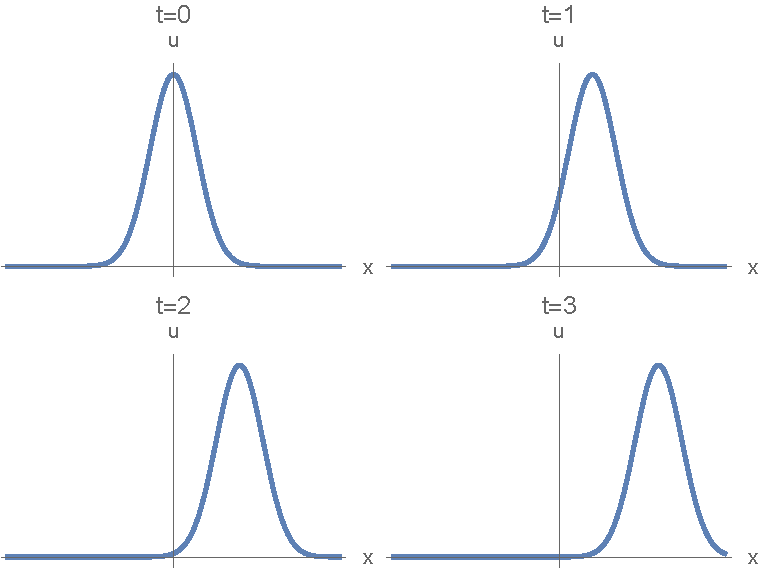
\includegraphics[width=0.8\textwidth]{images/travelling-plane-wave}
        \caption[travelling plane wave]{A plane wave, \(\exp(-(x - ct)^2)\), travelling to the right as time progresses.}
        \label{fig:travelling plane wave}
    \end{figure}
    
    Since both the left and right moving waves are travelling at the same speed, \(c\), which depends only on the value \(c\) in the original wave equation we see that the speed of the waves is independent of the particular form of \(F\) and \(G\).
    This is a special property of this equation, not all equations admitting travelling wave solutions like these do so in a way that makes the speed independent of the initial conditions.
    In applications the value of \(c\) will depend on the medium through which the wave is travelling.
    For example, the wave equation drops nicely out of Maxwell's equations, in which case the medium is the electromagnetic field and \(c = \sqrt{\varepsilon_0 \mu_0}\) turns out to be the speed of light.
    
    \section{Another Example}
    Consider the PDE
    \begin{equation}
        u_t \pm c u_x = 0.
    \end{equation}
    We can apply exactly the same method, introducing the variables \(X\) and \(T\), which gives
    \begin{equation}
        u_t + cu_x = -c\partial_Xu + c\partial_Tu + c(\partial_X u + \partial_T u) = 0 \implies \partial_T u = 0
    \end{equation}
    and
    \begin{equation}
        u_t - cu_x = -c\partial_Xu + c\partial_Tu - c(\partial_X u + \partial_T u) = 0 \implies \partial_X u = 0.
    \end{equation}
    We can then integrate these to get
    \begin{equation}
        u = f(T), \qand u = f(X)
    \end{equation}
    as our two solutions, so the solution to the original equation is
    \begin{equation}
        u(x, t) = f(x \mp ct)
    \end{equation}
    for an arbitrary function \(f\).
    
    As before we can interpret \(f(x - ct)\) as a right moving wave, and \(f(x - ct)\) as a left moving wave.
    So our solutions look like just a single right or left moving wave, rather than two waves moving in opposite directions.
    Again, the speed of either the left or right moving wave is \(c\), and this is independent of the initial profile of the wave.
    
    \section{Dispersive Term}
    We can modify the equation of the previous section by addition of an extra term, \(u_{xxx}\):
    \begin{equation}
        u_t + u_x + u_{xxx} = 0.
    \end{equation}
    We call this extra term the dispersive term, for reasons we'll explain shortly.
    We will find a solution to this by making the ansatz of harmonic waves, that is we posit that the solution is\footnote{If we want real solutions then we should instead consider \(\e^{i(kx - \omega t)} \pm \e^{-i(kx - \omega t)}\), but things are simpler if we just allow complex solutions.}
    \begin{equation}
        u(x, t) = \e^{i(kx - \omega t)}
    \end{equation}
    where \(k\) and \(\omega\) are some constants.
    The question is then under what conditions is this a solution to the equation in question?
    To answer this we simply substitute this into the equation, which we can do using
    \begin{equation}
        u_t = -i\omega\e^{i(kx - \omega t)}, \quad u_x = ik\e^{i(kx - \omega t)}, \qand u_{xxx} = (ik)^3\e^{-i(kx - \omega t)}.
    \end{equation}
    Then we have
    \begin{equation}
        [-i\omega + ik - ik^3]\e^{i(kx - \omega t)} = 0.
    \end{equation}
    Since the exponential is never zero we must have that the factor in front vanishes, and so
    \begin{equation}
        \omega(k) = k - k^3 = k(1 - k^2).
    \end{equation}
    This, and similar relations for other PDEs, are called the \defineindex{dispresion relation}.
    
    From this we know that our ansatz is a valid solution so long as \(\omega(k) = k(1 - k^2)\).
    We can then write the solution as
    \begin{equation}
        u(x, t) = \exp\{ik[x - (1 - k^2)t]\}.
    \end{equation}
    We can then see that this is a wave of speed \(1 - k^2\).
    In general, if we have a harmonic wave ansatz then the speed of the wave will be
    \begin{equation}
        c = \frac{\omega(k)}{k}.
    \end{equation}
    
    The general solution is a linear superposition of harmonic waves with different values of \(k\), such as
    \begin{equation}
        u(x, t) = \sum_{n} A(k_n) \e^{ik_n(x - (1 - k_n^2)t)}.
    \end{equation}
    In the limit we may instead take
    \begin{equation}
        u(x, t) = \int A(k) \e^{ik(x - (1 - k^2)t)} \dd k.
    \end{equation}
    For simplicity we'll consider the first solution with the sum.
    Notice that different values of \(k\) mean different speeds.
    Suppose we start with three different values of \(k\) with three arbitrary amplitudes.
    Even if we start with all three waves localised at the same position after some time they will spread out.
    This is what we call \defineindex{dispersion}, and it's why we call \(u_{xxx}\) a dispersive term, and \(\omega(k) = k(1 - k^2)\) a dispersion relation, because any non-constant dispersion relation will result in dispersive behaviour.
    This is shown in \cref{fig:dispersion of plane waves}.
    
    \begin{figure}
        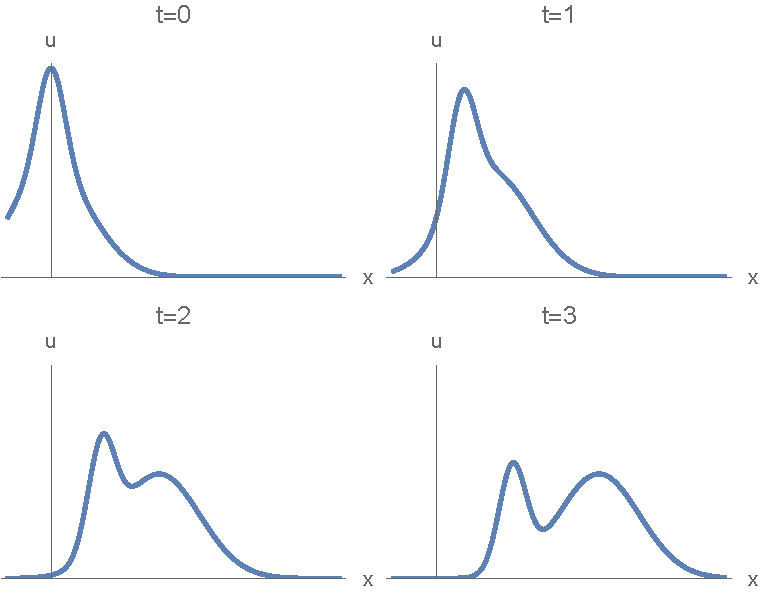
\includegraphics[width=0.8\textwidth]{images/dispersion-of-plane-waves}
        \caption[Dispersion of plane waves]{A solution consisting of two travelling waves with different speeds, which initially start at the same position and spread out as time progresses and the waves move right at different speeds. Note that the profile of these waves is not harmonic, but instead a Gaussian.}
        \label{fig:dispersion of plane waves}
    \end{figure}
    
    The fact that the individual waves spread out forces us to be a bit more specific about what we mean by velocity.
    There are in fact two different speeds that are important, which just happened to be equal up until now.
    These are
    \begin{itemize}
        \item the \defineindex{phase velocity}, \(c = \omega(k)/k\), which measures the speed of a single wave;
        \item the \defineindex{group velocity}, \(\groupVelocity = \difs{\omega(k)}{k}\), which measures the speed of the wave packet (the combination of all the single waves).
    \end{itemize}
    In our case
    \begin{equation}
        c = \frac{\omega(k)}{k} = 1 - k^2, \qqand \groupVelocity = \diff{\omega(k)}{k} = 1 - 3k^2.
    \end{equation}
    Note that usually, in physically realistic systems, \(\groupVelocity \le c\).
    If we think of the wave as carrying some energy then \(\groupVelocity\) is the speed that this energy is carried at.
    
    \begin{app}{}{}
        AM radio works by using electromagnetic waves (specifically radio waves) travelling at the speed of light.
        However, the signal is encoded in the wave packet by changing the amplitude, and the wave packet travels at a speed less than the speed of light, which allows this information to still be read by an electrical component, which could not deal with the speed of light.
        In fact, AM stands for amplitude modulation because this is how it works.
        This can be contrasted with FM radio, where FM stands for frequency modulation, in which the information is transmitted by varying the frequency of the waves and therefore the speed of the waves isn't important because the rate of frequency modulation is the important speed.
    \end{app}
    
    Note that for the original wave equation the dispersion relation is \(\omega(k) = ck\), and so \(\groupVelocity = \omega'(k) = c\), so the group velocity and phase velocity are the same here.
    
    \section{Dissipative Term}
    We could instead have modified the equation by adding an extra term\footnote{We choose \(-u_{xx}\), as opposed to \(+u_{xx}\) as this is the more common case in physical situations.}, \(-u_{xx}\), to get
    \begin{equation}
        u_t + u_x - u_{xx} = 0.
    \end{equation}
    We make the same ansatz,
    \begin{equation}
        u(x, t) = \e^{i(kx - \omega t)},
    \end{equation}
    and using
    \begin{equation}
        u_{xx} = (ik)^2\e^{i(kx - \omega t)}
    \end{equation}
    substituting into the equation we have
    \begin{equation}
        [-i\omega + ik - k^2] \e^{i(kx - \omega t)} = 0.
    \end{equation}
    Since the exponential is never zero we must have that the factor in front vanishes, and so
    \begin{equation}
        \omega(k) = k - ik^2.
    \end{equation}
    We may then write the solution as
    \begin{equation}
        u(x, t) = \e^{i k(x - t)} \e^{-k^2t}.
    \end{equation}
    The first exponential here is oscillatory, and the second decays to zero as time progresses.
    The result is that we have an oscillation which decays to zero amplitude.
    This is shown in \cref{fig:dissipative wave}
    
    \begin{figure}
        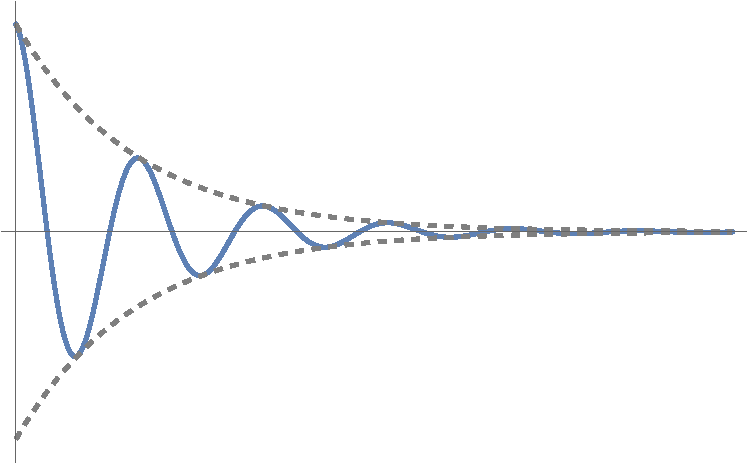
\includegraphics[width=0.8\textwidth]{images/dissipative-wave}
        \caption[dissipative wave]{A harmonic wave solution to a dissipative equation. Note that the plot shows the motion of a fixed point, say that at \(x = 0\), as it oscillates in time. The amplitude of the oscillations decays exponentially.}
        \label{fig:dissipative wave}
    \end{figure}
    
    \chapter{Nonlinear Equations}
    \section{Simple Nonlinear Example}
    \label{sec:simple nonlinear example}
    Consider the equation
    \begin{equation}
        u_t + (1 + u)u_x = 0.
    \end{equation}
    This is a nonlinear PDE due to the \(uu_x\) term.
    Despite this it still has an exact solution, which can be found using the \enquote{method of characters}.
    We won't go into details about how this works here.
    The method of characters solves equations of the form
    \begin{equation}
        u_t + A(u) u_x = 0
    \end{equation}
    for some function \(A\).
    Such equations are sometimes called \defineindex{quasilinear} since they are linear in the derivatives of \(u\), but not in \(u\) itself.
    In our case \(A(u) = 1 + u\).
    The method consists of solving the equation
    \begin{equation}
        \diff{x}{t} = A(u)
    \end{equation}
    while treating \(u\) as a constant.
    In our case this means solving
    \begin{equation}
        \diff{x}{t} = 1 + u
    \end{equation}
    with \(u\) constant.
    We can integrate this equation to get the solution
    \begin{equation}
        x = (1 + u)t + C
    \end{equation}
    where \(C\) is some constant of integration.
    We then solve this for \(C\), giving
    \begin{equation}
        C = x - (1 + u)t.
    \end{equation}
    We call this these the \define{characteristic line}\index{characteristic line}.
    The solution to the original equation is then
    \begin{equation}
        u(x, t) = f(C) = f(x - (1 + u)t)
    \end{equation}
    for an arbitrary function, \(f\).
    Notice that \(u\) appears on both sides of this equation, so this is an implicit function solution for \(u\), rather than an explicit one.
    Nevertheless we can still tell quite a lot about this wave qualitatively.
    Setting \(t = 0\) we have \(u(x, 0) = f(x)\), and so \(f\) is determined by the initial profile of the wave.
    We can see that \(u\) takes the form of a wave travelling to the right of speed \(1 + u\).
    The unusual thing here is that the speed of the wave actually varies in space, and further, the speed of the wave a point depends on the height of the wave at that point.
    For an initial Gaussian profile the speed of the wave at \(t = 0\) at several positions is shown in \cref{fig:height dependent speed}.
    
    \begin{figure}
        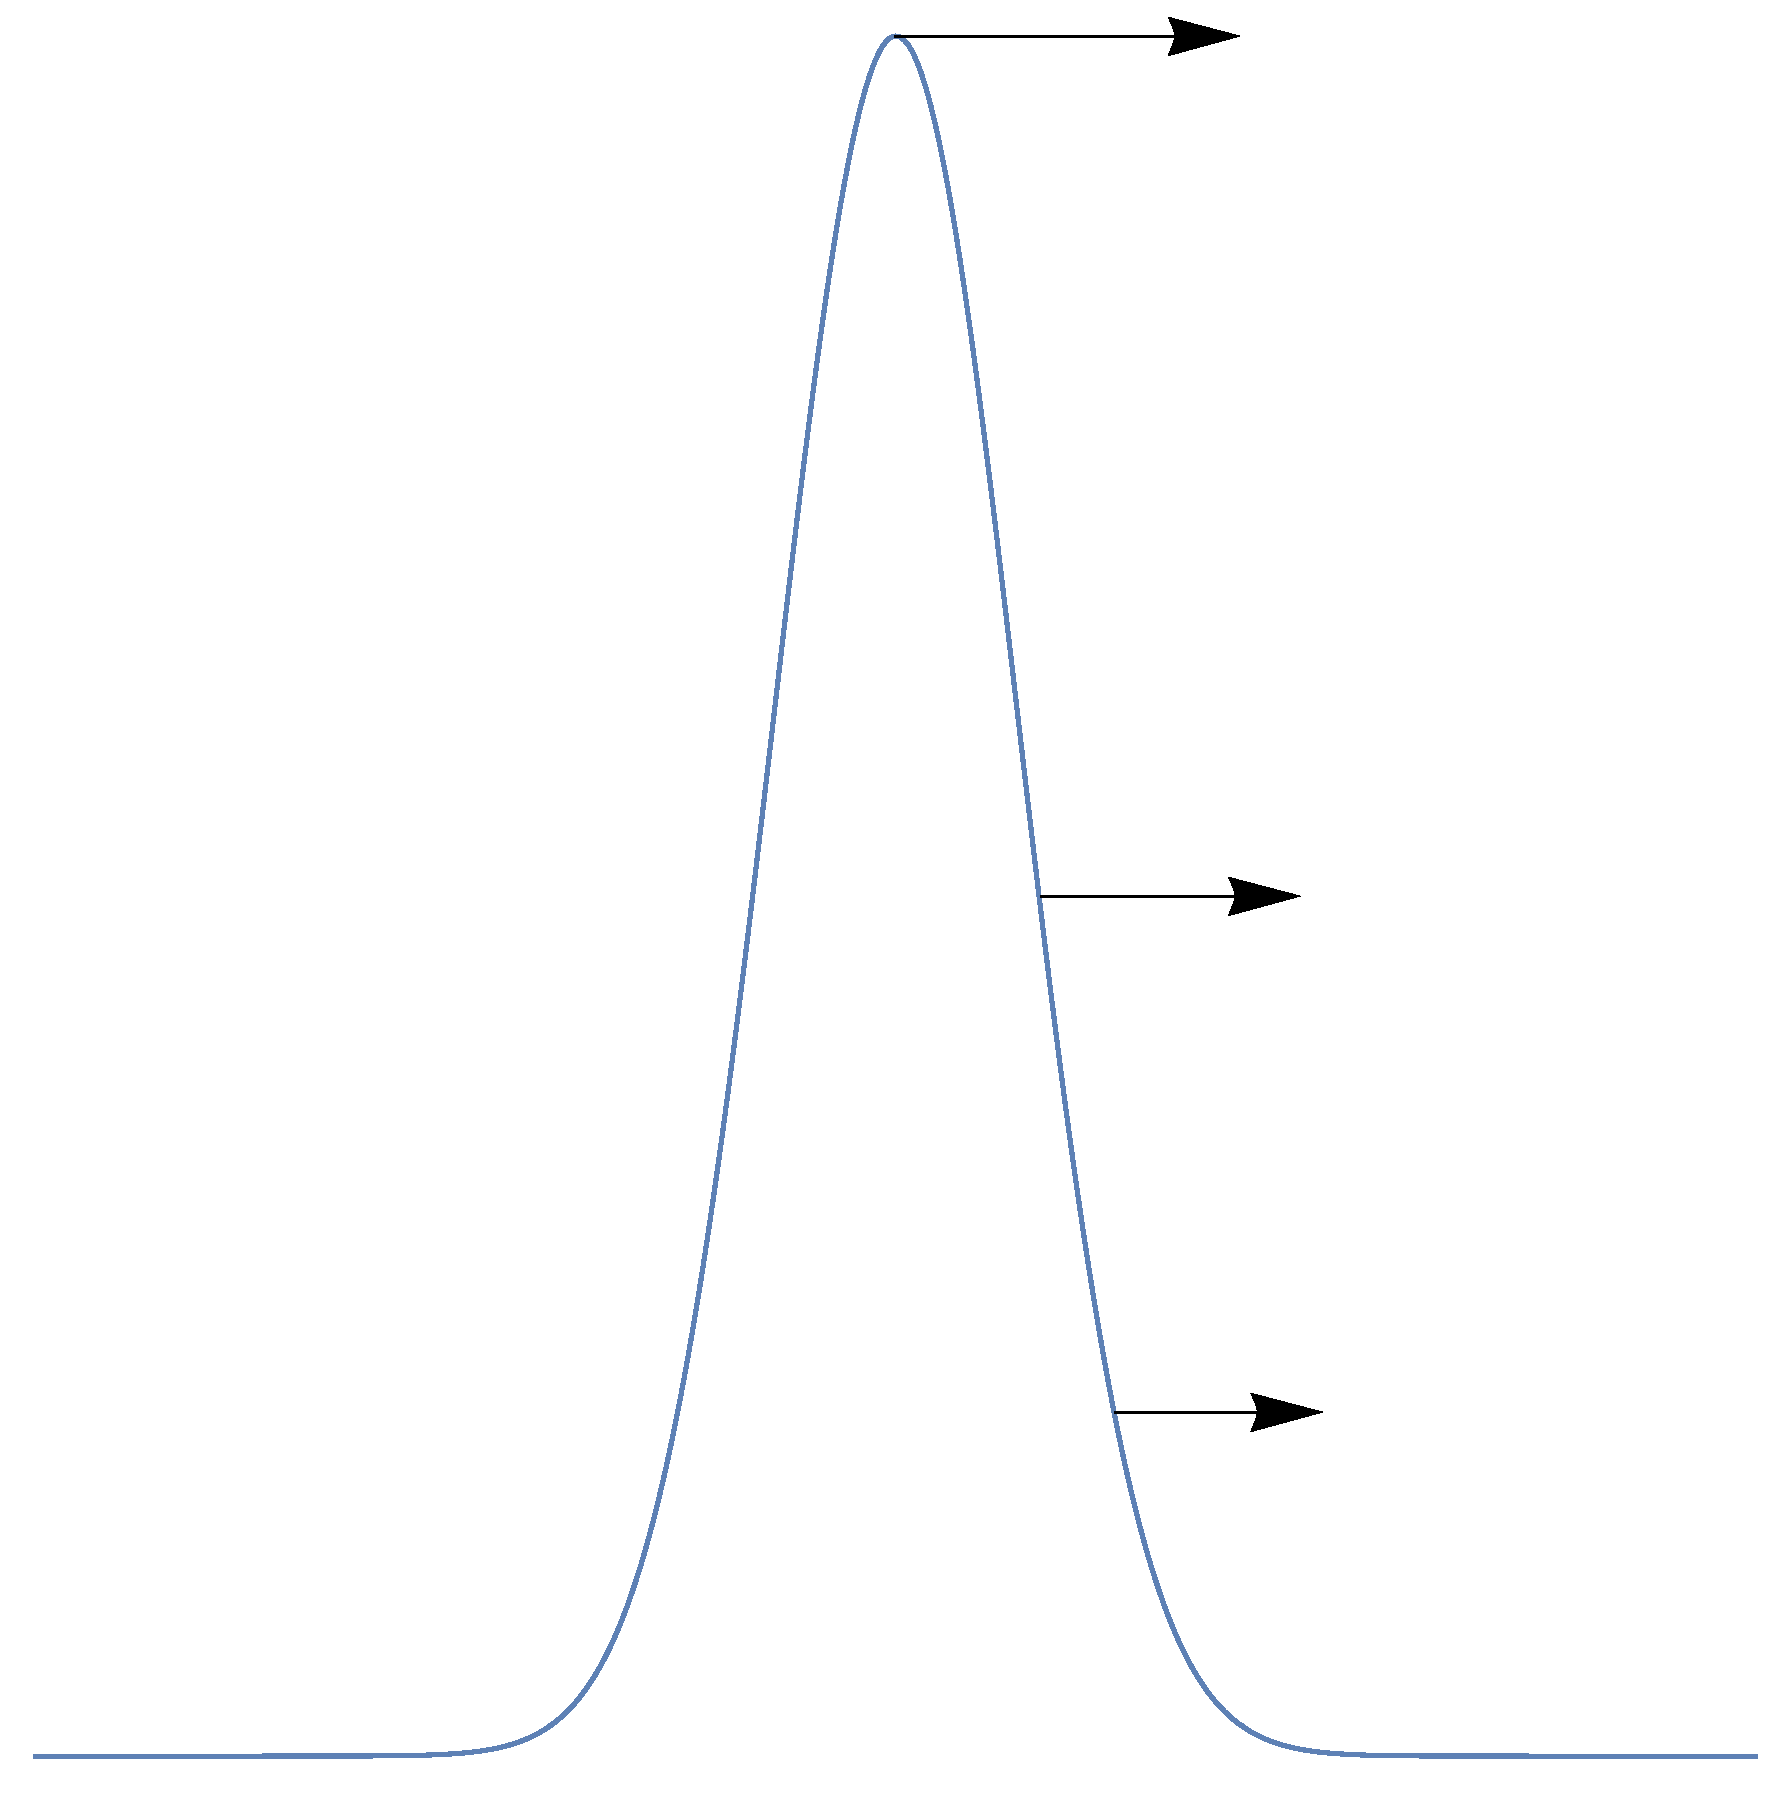
\includegraphics[width=0.8\textwidth]{images/height-dependent-speed}
        \caption[height dependent speed]{A wave in which the speed depends on the height of the wave. The arrows are the velocity vectors for the parts of the wave they start at.}
        \label{fig:height dependent speed}
    \end{figure}
    
    Now consider what happens to this wave as time progresses.
    The peak of the wave will move faster than the base of the wave, so the wave starts to bunch up to the right.
    Eventually the peak overtakes the wave, and the wave breaks.
    This happens at the point at which \(u_x\) diverges, when the right hand side of the wave becomes vertical.
    After this point there are two options for what we can do.
    The function \(u\) becomes multi-valued after the wave breaks.
    If the physical situation allows, such as for a water wave where \(u\) is the height of any and all air-water boundaries, this is fine, we see waves break like this all the time.
    This is shown in \cref{fig:breaking wave}.
    For physical situations where multi-valued functions aren't allowed we can instead modify the solution to have a a sudden jump down to the base at some point, of course these types of discontinuous solutions come with their own problems.
    
    \begin{figure}
        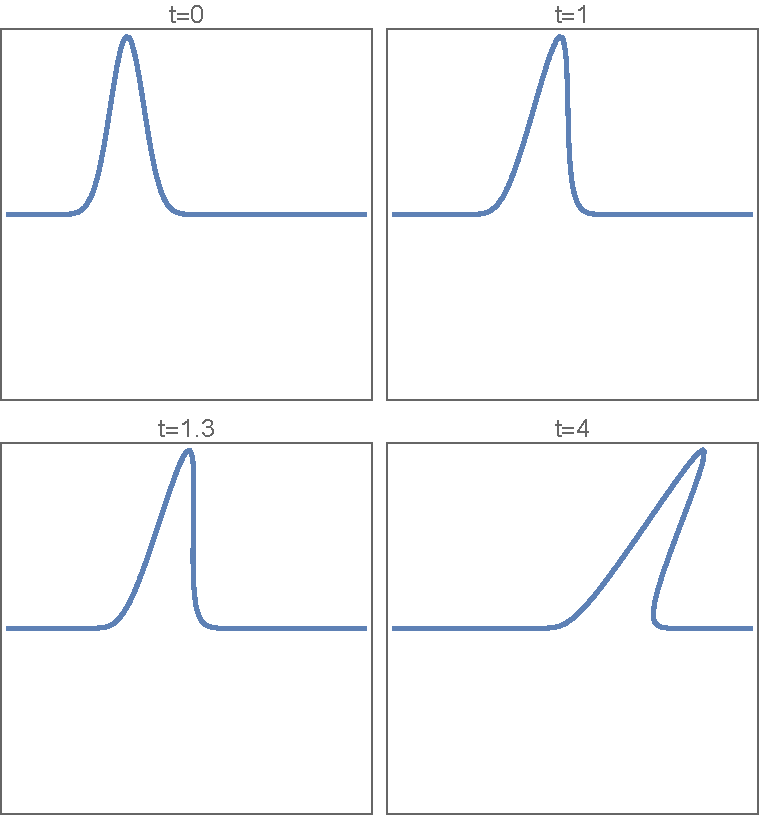
\includegraphics[width=0.8\textwidth]{images/breaking-wave}
        \caption[breaking wave]{A wave with an initial Gaussian profile breaking, the break occurs approximately at the time of the third frame, and after the break the function becomes multi-valued.}
        \label{fig:breaking wave}
    \end{figure}
    
    \section{Burger's Equation}
    A surprising fact is that some nonlinear equations can be made linear by a nonlinear change of variables.
    This is rare, but one example is \defineindex{Burger's equation}:
    \begin{equation}
        u_t + (1 + u)u_x - u_{xx} = 0.
    \end{equation}
    This is nonlinear, and as such if \(u_1\) and \(u_2\) are two solutions \(u_1 + u_2\) is, in general, not a solution.
    Notice that this is just the nonlinear equation from the previous section with an added dissipative term.
    
    The change of variables we want to consider here is called the \defineindex{Cole--Hopf transformation}, and it's given by
    \begin{equation}
        u = A(\log \varphi)_x = A \partial_x \log \varphi = A\frac{\varphi_x}{\varphi}
    \end{equation}
    for some constant \(A\), which we choose so that the resulting equation is linear.
    It's best if we proceed in steps here.
    First we do a transformation \(u = \psi_x\), so our equation becomes
    \begin{equation}
        \psi_{tx} + (1 + \psi_x)\psi_{xx} - \psi_{xxx} = 0
    \end{equation}
    which expands to
    \begin{equation}
        \psi_{tx} + \psi_{xx} + \psi_x \psi_{xx} - \psi_{xxx} = 0.
    \end{equation}
    We can integrate this, by recognising that
    \begin{equation}
        \psi_x\psi_{xx} = \frac{1}{2}\diffp{}{x}(\psi_x^2)
    \end{equation}
    and so this integrates to
    \begin{equation}
        \psi_t + \psi_x + \frac{1}{2}\psi_x^2 - \psi_{xx} = 0.
    \end{equation}
    Now take \(\varphi = A\log \psi\) and we have
    \begin{equation}
        \psi_t = \frac{A \varphi_t}{\varphi}, \quad \psi_x = \frac{A \varphi_x}{\varphi}, \qand \psi_{xx} = -\frac{A\varphi_x^2}{\varphi^2} + \frac{A\varphi_{xx}}{\varphi}.
    \end{equation}
    Substituting this into the equation above we get
    \begin{equation}
        \frac{A}{\varphi} \left[ \varphi_t + \varphi_x + \frac{1}{2}\frac{A\varphi_x^2}{\varphi} - \frac{\varphi_x^2}{\varphi} + \varphi_{xx} \right] = 0.
    \end{equation}
    Assuming that \(A \ne 0\) we therefore have
    \begin{equation}
        \varphi_t + \varphi_x + \left( \frac{A}{2} - 1 \right) \frac{\varphi_x^2}{\varphi} + \varphi_{xx} = 0.
    \end{equation}
    Thus, by taking \(A = 2\) we get the linear equation
    \begin{equation}
        \varphi_t + \varphi_x + \varphi_{xx} = 0.
    \end{equation}
    This is exactly the dissipative equation we had before, the \(+\) instead of the \(-\) on the dissipative term just means we end up with \(\e^{+k^2t}\), so rather than dissipating the amplitude grows exponentially.
    
    It should be noted that the ability to make a nonlinear equation linear like this is rare.
    Note also that the original equation is still nonlinear, in particular it doesn't have the linear superposition property.
    However, we do have linear superposition of solutions, \(\varphi_1\) and \(\varphi_2\), to the linear version.
    It's just that \(A(\log(\varphi_1 + \varphi_2))_x \ne A(\log \varphi_1)_x + A(\log \varphi_2)_x\) in general, and so this superposition doesn't give a superposition in the original variables.
    
    \section{KdV Equation}
    The \defineindex{KdV equation}, named for two mathematicians, Korteveg and de Vries, will be one of the main equations we study.
    It most naturally arises at this point as the same equatoin as above, but with a dispersive term, instead of a dissipative one.
    That is, the KdV equation is
    \begin{equation}
        u_t + (1 + u) u_x - u_{xx} = 0.
    \end{equation}
    
    By rescaling \(x\), \(t\), and \(u\), as well as translations in \(u\), there are several ways to write this equation.
    The most standard form is
    \begin{equation}
        u_t - 6uu_x + u_{xxx} = 0.
    \end{equation}
    However, many forms are common, with different forms lending themselves to different areas and methods.
    The factor of \(6\) is mostly just convention, it's possible to write the equation in this form with any nonzero coefficients we like by rescalings.
    
    The KdV equation will be important for our study because it is an integrable equation with \enquote{multi-soliton solutions}.
    We'll define what this means later, but for now we look at one particular solution, which is the single-soliton solution.
    We will derive this solution later, for now we just state it:
    \begin{equation}
        u(x, t) = 2k^2 \sech^2(k(x - 4k^2 t + x_0))
    \end{equation}
    for some constant \(x_0\).
    
    Recall that \(\sech a = 1/\cosh a\).
    It just so happens that \(\sech a\) is localised with a peak at \(0\), and squaring it just makes a similar graph with a narrower peak.
    Plots of \(\cosh a\), \(\sech a\), and \(\sech^2 a\) are shown in \cref{fig:sech squared}.
    Notice that since \(\cosh a \ge 1\) for all \(a \in \reals\) we have \(0 \le \sech^2a \le 1\) for all \(a \in \reals\).
    The \(\sech^2\) profile is very typical of single soliton solutions.
    
    \begin{figure}
        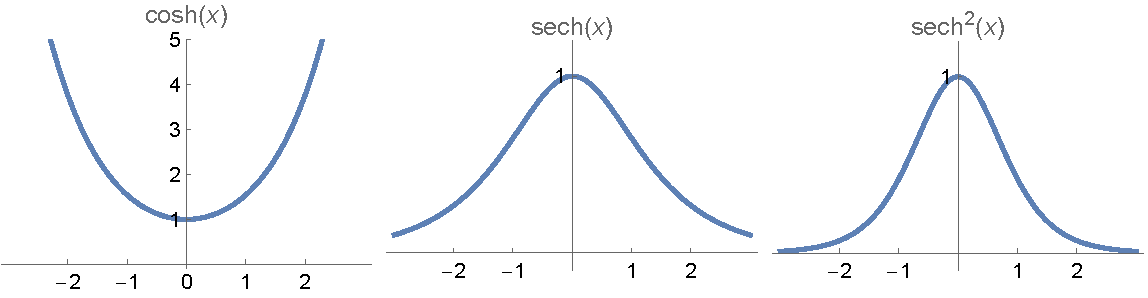
\includegraphics[width=0.8\textwidth]{images/sech}
        \caption[\(\sech^2 a\)]{Plot of \(\cosh a\), \(\sech a\), and \(\sech^2 a\).}
        \label{fig:sech squared}
    \end{figure}
    
    The speed at which this wave travels is \(4k^2\), and the amplitude of the wave is \(2k^2\), so the speed of the soliton depends on its height.
    Note that this is not like the previous height dependence, where the speed of the wave varied with position.
    Here the speed of the wave depends only on the maximum value of the wave.
    This gives us an important general principle, which is that taller solitons move faster.
    
    There is no linear superposition in the KdV equation.
    If \(u_1\) and \(u_2\) are two solutions, say two one-soliton solutions of the \(\sech^2\) profile above with different values of \(k\) then \(u_1 + u_2\) is, in general, not a solution.
    
    \chapter{Travelling Wave Solutions}
    \section{Method}
    There is a particular method of finding certain wave solutions to PDEs based on the solutions to the wave equation.
    We take inspiration from the solutions \(F(x - ct)\) and \(G(x + ct)\) for the wave equation and we posit the existence of a solution \(u = f(x - ct)\) for some unknown value, \(c\).
    We then substitute this into the one-dimensional PDE for \(u(x, t)\) and the result is an ODE in \(f\).
    We call the solutions found this way \define{travelling wave solutions}\index{travelling wave solution}.
    
    In general this ODE will only have solutions for certain values of \(c\), and the solutions we find are only particular solutions, most PDEs have solutions that aren't purely travelling waves.
    
    \section{Simple Nonlinear Example}
    Consider the equation
    \begin{equation}
        u_t + (1 + u)u_x = 0.
    \end{equation}
    We saw in \cref{sec:simple nonlinear example} that this has general solutions \(f(x - (1 + u)t)\), which have the property that points higher up the wave travel faster.
    We will now look for travelling wave solutions to this equation.
    
    Let \(u(x, t) = f(x - ct)\) and introduce the variable \(\xi = x - ct\).
    Then we have
    \begin{equation}
        u_x = \diffp{}{x} f(x - ct) = f'(x - ct) = f'(\xi)
    \end{equation}
    and
    \begin{equation}
        u_t = \diffp{}{t} f(x - ct) = -cf'(x - ct) = -cf'(\xi).
    \end{equation}
    Substituting these into the PDE we get the ODE
    \begin{equation}
        -cf_\xi + (1 + f)f_\xi = 0. 
    \end{equation}
    Rearranging this we get
    \begin{equation}
        (1 - c + f)f_\xi = 0
    \end{equation}
    and so we have two cases:
    \begin{itemize}
        \item \(f_\xi = 0\), in which case \(f = \const\); and
        \item \(1 - c + f = 0\), in which case \(f = 1 - c = \const\).
    \end{itemize}
    We see that \(c\) can take on any real value, and the result is always that \(f\) is constant.
    So, the only travelling wave solutions are constant.
    
    This shouldn't be too surprising.
    When solving for travelling wave solutions we take \(c\) to be constant, and \(c\) is the speed of the travelling wave.
    We have seen already that the speed of wave-like solutions to this equation have speeds depending on the height of the wave at that position.
    So, the only way for the whole wave to travel at the same speed is if the whole wave is at the same height, that is if the wave is constant.
    
    \subsection{Adding in a Source Term}
    Consider the modified equation
    \begin{equation}
        u_t + (1 + u)u_x = V(u)
    \end{equation}
    where \(V\) is an arbitrary function.
    We call \(V\) a source term, because in, say, electromagnetism adding such a term to Laplace's equation (\(\laplacian \varphi = 0\)) to produce Poisson's equation (\(\laplacian \varphi = V(u)\)) this term represents a charge density, which is then a source of the electric field.
    
    We can proceed with our attempt to find travelling wave solutions to this equation.
    Making the same transformation as before we get
    \begin{equation}
        -cf_\xi + (1 + f)f_\xi = V(f).
    \end{equation}
    This ODE for \(f\) is actually separable, and the solution is thus
    \begin{equation}
        \int \frac{1 + c - f}{V(f)} \dd{f} = \int \dl{\xi} = \xi + \const.
    \end{equation}
    
    There are two problems that may arise at this point:
    \begin{itemize}
        \item We need to actually be able to do this integral, which is far from guaranteed.
        \item If we successfully perform the integral then we will have expressed \(\xi\) (plus a constant) as a function of \(f\).
        This gives an implicit formula for \(f\) which we need to invert this if we want an explicit definition.
    \end{itemize}
    This shows just some of the problems that can arise when looking for travelling wave solutions of even fairly simple nonlinear PDEs.
    A more complicated PDE could give rise to an ODE for \(f\) which cannot be so easily solved, adding to the difficulty of finding travelling wave solutions.
    
    
    % Appdendix
    %	\appendixpage
    %	\begin{appendices}
        %	
        %	\end{appendices}
    
    \backmatter
    \renewcommand{\glossaryname}{Acronyms}
    \printglossary[acronym]
    \printindex
\end{document}